\documentclass[12pt]{article}
\usepackage[margin=1in]{geometry}
\usepackage{amsmath,amssymb,amsthm}
\usepackage{mathtools}
\usepackage{hyperref}
\usepackage{bm}
\usepackage{natbib}
\usepackage{authblk}
\usepackage{algorithm}
\usepackage{algpseudocode}
\usepackage{booktabs}
\usepackage{graphicx}
\graphicspath{{figures/}}

\newcommand{\cG}{\mathcal{G}}
\newcommand{\cN}{\mathcal{N}}
\newcommand{\cE}{\mathcal{E}}
\newcommand{\cX}{\mathcal{X}}
\newcommand{\cB}{\mathcal{B}}

\DeclareMathOperator*{\argmin}{arg\,min}
\DeclareMathOperator*{\argmax}{arg\,max}

\newtheorem{proposition}{Proposition}
\newtheorem{assumption}{Assumption}
\newtheorem{remark}{Remark}
\newtheorem{lemma}{Lemma}

\title{A Semiparametric Perturbed Utility \\
Route Choice Model}
\author{%
Mogens Fosgerau\thanks{University of Copenhagen} \quad
Xuhang Liu\thanks{EPFL} \\
Rui Yao\thanks{Technion} \quad
Kenan Zhang\thanks{EPFL}%
}
\date{\today}


\begin{document}
\maketitle

\begin{abstract}
We develop a semiparametric estimator for the perturbed utility route choice (PURC) model in which the perturbation function is a polynomial whose shape parameters are estimated from data alongside the utility parameters. The natural estimation criterion is the Fenchel-Young loss, but on disaggregate trip-level data its score for the shape parameters is biased: the perturbation is evaluated at binary link-incidence vectors, collapsing the nonlinear basis functions that distinguish shape parameters to a common linear form. We resolve this by replacing the perturbation term with falling-factorial U-statistics computed from repeated trips within origin-destination pairs, which provide unbiased estimates of the powers of the optimal flow. The resulting debiased Fenchel-Young loss is jointly convex in all parameters and has unbiased scores at the true parameter. We establish $\sqrt{B}$-consistency and asymptotic normality of the estimator. A simulation study and an empirical application to Shenzhen taxi trajectory data demonstrate the approach.
\end{abstract}

\begin{itemize}
    \item MF to write illustration of activation function.
    \item Note for the future: the model setup can generalize to arbitrary budget sets in $[0,1]^n$ and observed choices $y\in \{0,1\}^n $ 
    \item MF: We need a better motivation for the paper. Something along these lines, perhaps: Many prediction models have the form $x=\argmin_{x\in B}\{v'x+F(x)\}.$ (ARUM, PURC, ). The shape of $F$ is important for predictions: controls sparsity and it controls the sensitivity of $x$ to $v$.  So it is of interest to be able to estimate the shape of $F$ from data. This paper presents such an estimator. 
    \item $F$ may be motivated as a regularizer. But in many cases, it is better thought of as an integral part of the model rather than an ad hoc addition: when the behavior that the model is intended to describe is inherently dispersed. 
\end{itemize}

\section{Introduction}\label{sec:introduction}

This paper develops a semiparametric estimator for the perturbed utility route choice (PURC) model of \citet{fosgerau2022perturbed, fosgerau2023bikeability}. In the PURC model, a traveler chooses a flow $x$ over network links to maximize a perturbed utility $v^\top x - F(x)$, where $v$ is a vector of link utilities, $x$ is a vector of link flows, and $F$ is a strictly convex perturbation function that regularizes the flow. We specify $F$ flexibly as a polynomial whose coefficients are estimated from data.

The convexity of the perturbation function controls how much it penalizes the concentration of flow. Thus, the shape of the function matters substantially for the predictions of the PURC model. This paper makes the shape of the perturbation function an empirical issue rather than a modelling choice. 


The PURC model can predict sparsity by design: travelers rule out implausible links rather than assigning them small-but-positive probability. This makes the model behaviorally appealing for route choice on large networks. 

We estimate the model using a debiased version of the Fenchel-Young (FY) loss \citep{blondel_learning_2020, lin_fenchel-young_2026}. The standard FY loss is the natural fit for a perturbed utility model: it is convex in parameters, finite everywhere even under sparsity, and has a clean residual-form gradient. 

However, the perturbation function plays two roles in the FY loss: it defines the estimation criterion, but it also contains shape parameters to be estimated. This dual role introduces a bias in the score for the shape parameters. The issue is that the FY loss evaluates the perturbation at the observed link-incidence vector, which is binary. Since all powers of a binary variable coincide, $y^l = y$ for $l \geq 1$, the nonlinear basis functions that distinguish different shape parameters collapse to a common linear form, and the score cannot separate them.

We resolve this issue by debiasing the FY loss: replacing the perturbation evaluated at the binary observation with a corrected term that restores the missing curvature information. The corrected term uses falling-factorial U-statistics computed from repeated trips within origin-destination (OD) pairs. Under the model, the count of trips traversing a link is binomial, and the falling-factorial ratio $n^{(l)}/D^{(l)}$ is the unique minimum-variance unbiased estimator of the $l$th power of the link flow. Substituting these U-statistics for the powers of $y$ in the primal term of the FY loss yields a debiased objective that is jointly convex in utility and shape parameters and has unbiased scores at the true parameter vector. The resulting estimator is a single convex optimization problem with consistent estimates of both sets of parameters.



The present paper generalizes this setting to allow the shape of a perturbation kernel to be estimated. Incidentally, the present paper shows the FY loss criterion applies directly to disaggregate trip-level data with given link perturbation functions.



\subsection{Related literature}

The literature on route choice is extensive; see \citet{prato_route_2009} for a review. Most studies treat route choice as a discrete choice among routes, which creates the challenge that the number of feasible routes is enormous. Research has therefore focused on constructing choice sets with good coverage to avoid bias and on developing models with realistic substitution patterns.

A newer line of research considers recursive models, where travelers choose paths link by link in a Markovian fashion. Early work addressed the assignment problem \citep{Dial1971, bell_alternatives_1995, baillon_markovian_2008}. Subsequent studies introduced the recursive logit model and its generalizations \citep{fosgerau_link_2013, Mai2015a, mai_method_2016}. However, applying recursive logit to large networks remains challenging due to the need to invert large matrices; see \citet{zimmermann_tutorial_2020} for a tutorial.

The PURC model \citep{fosgerau2022perturbed, fosgerau2023bikeability} departs from the discrete choice paradigm by modeling travelers as maximizing a perturbed utility function \citep{fosgerau2012theory}. It requires no choice set and uses the entire network directly. Substitution patterns arise from the network structure via a perturbation function defined as a sum of convex link-flow functions. \citet{fosgerau_convex_2026} develop the convex duality framework that underlies the computational approach used in this paper. \citet{yao_perturbed_2024} propose a fast algorithm for computing equilibrium assignment in large networks, and \citet{fosgerau_sensitivity_2025} develop sensitivity analysis for the PURC equilibrium.

The Fenchel-Young loss was introduced in the machine learning community by \citet{blondel_learning_2020} as a convex estimation criterion for regularized prediction functions, which are equivalent to perturbed utility demand functions. \citet{lin_fenchel-young_2026} apply this loss to the estimation of perturbed utility discrete choice models, and \citet{yin_fenchel-young_2026} apply it to route choice on aggregate link-flow data.
The present paper introduces the semiparametric perturbation and the U-statistic debiasing that makes Fenchel-Young estimation of the shape parameters consistent. \citet{fosgerau_estimating_2024} propose a different estimator for the standard PURC model on trip-level data, based on a projected first-order condition, which can similarly be extended to the semiparametric setting and does not require within-OD repeats, but provides only local convergence guarantees. The debiased FY estimator is globally convex, making it attractive when OD pairs have enough repeated trips to allow the shape parameters to be estimated with adequate precision. 

The remainder of the paper is organized as follows. Section~\ref{sec:model} introduces the PURC model, the data-generating process, and the semiparametric perturbation kernel. Section~\ref{sec:duality_conjugate} presents the duality framework used for computation. Section~\ref{sec:FYloss_bias} introduces the standard FY loss and establishes its bias for shape parameters. Section~\ref{sec:debiased} constructs the debiased FY loss and establishes its properties. Section~\ref{sec:estimator} defines the estimator and establishes consistency and asymptotic normality. Section~\ref{sec:algorithm} describes the algorithm. Sections~\ref{sec:simulation} and~\ref{sec:application} present a simulation study and an empirical application to Shenzhen taxi data, respectively. Section~\ref{sec:conclusion} concludes.

\section{Model}\label{sec:model}

\subsection{Network and demand}

Let $\cG = (\cN, \cE)$ be a strongly connected directed network with nodes $\cN$ and links $\cE$. Let $A \in \mathbb{R}^{|\cN| \times |\cE|}$ denote the node-link incidence matrix, with $A_{i,(i,j)} = 1$, $A_{j,(i,j)} = -1$, and zero elsewhere. For each link $(i,j) \in \cE$, let $z_{(i,j)} \in \mathbb{R}^K$ be a vector of observed attributes and $\ell_{(i,j)} > 0$ the link length.

A trip is characterized by a demand vector $b \in \mathbb{R}^{|\cN|}$ satisfying $b_o = 1$ at the origin $o$, $b_d = -1$ at the destination $d$, and $b_i = 0$ otherwise.

\subsection{The basic PURC problem}

Let $v \in \mathbb{R}^{|\cE|}$ be a vector of link utilities and let $F(\cdot\,; \gamma) \colon \mathbb{R}^{|\cE|} \to \mathbb{R} \cup \{+\infty\}$ be a separable, strictly convex perturbation function parameterized by $\gamma \in \mathrm{int}( \Gamma)$, where $\Gamma$ is a closed convex set, with $F(x; \gamma) = \sum_{(i,j) \in \cE} F_{(i,j)}(x_{(i,j)}; \gamma)$ and $F_{(i,j)}(0; \gamma) = F'_{(i,j)}(0; \gamma) = 0$ for all $(i,j) \in \cE$. The specific functional form of $F$ is given in Section~\ref{sec:perturbation} below.


Given demand $b$, the optimal flow is
\[
    x^*_b(\theta) = \argmax_{x:\, Ax = b,\, x \geq 0}
        \bigl\{ v(\beta)^\top x - F(x; \gamma) \bigr\},
\]
where $\theta = (\beta, \gamma) \in \mathbb{R}^K \times \Gamma$.
Strict convexity of $F$ ensures a unique optimum whenever the feasible set is nonempty.

\begin{assumption}[Negative link utilities]\label{ass:neg_utility}
    The link utilities satisfy $v_{(i,j)} < 0, \; \forall (i,j) \in \cE$.
\end{assumption}
This assumption ensures that the optimal flow carries no cycles, so the active subnetwork $\{(i,j) : x^*_{(i,j)} > 0\}$ is acyclic \citep{fosgerau2022perturbed}. Acyclicity implies that each link carries at most one unit of flow, so $x^*_{(i,j)} \in [0, 1]$ for all links. The perturbation $F$ therefore need only be specified on $[0, 1]^{|\cE|}$; behavior outside this domain is irrelevant for the model.

Link utilities are assumed linear in a parameter
$\beta \in \mathbb{R}^K$:
\[
    v_{(i,j)}(\beta) = \beta^\top z_{(i,j)}.
\]
The condition $v_{(i,j)}(\beta_0) < 0$ for all links is not enforced during estimation but verified at the estimate.

\subsection{Data-generating process and moment identity}\label{sec:dgp}

We observe $D$ trips grouped by OD pair. Let $\cB$ denote the set of distinct OD pairs, with $|\cB| = B$, and let $D_b$ denote the number of trips observed for OD pair $b$, so $D = \sum_b D_b$ is the total number of trip observations.

\begin{assumption}[Data-generating process]\label{as:dgp}
There exists a true parameter $\theta_0 = (\beta_0, \gamma_0)$ such that, conditional on $b$, the trips $\{y_{b,d}\}_{d=1}^{D_b}$ for OD pair $b$ are i.i.d.\ realizations of the random-walk closure of the basic PURC problem at $\theta_0$: starting at the origin, the traveler selects the next link at each node with probability proportional to $x^*_{(i,j),b}(\theta_0)$, terminating at the destination.
\end{assumption}

The resulting link-incidence vectors satisfy $y_{b,d} \in \{0, 1\}^{|\cE|}$ and the moment identity
\begin{equation}\label{eq:moment-identity}
    \mathbb{E}[y_{(i,j),b,d} \mid b, \theta_0] = x^*_{(i,j),b}(\theta_0)
\end{equation}
for all $(i,j) \in \cE$, $b \in \cB$, $d = 1, \ldots, D_b$. For each link $(i,j)$ and OD pair $b$, let $n_{(i,j),b} = \sum_{d=1}^{D_b} y_{(i,j),b,d}$ be the number of trips that traverse link $(i,j)$, and let $\bar{y}_b = D_b^{-1} \sum_{d=1}^{D_b} y_{b,d}$ be the within-OD sample mean flow. Under Assumption~\ref{as:dgp}, the marginal count $n_{(i,j),b}$ is $\text{Binomial}(D_b, x^*_{(i,j),b})$.

\subsection{Semiparametric link perturbation on the unit interval}\label{sec:perturbation}

We refer to the model as semiparametric because the perturbation kernel $h$ is not assumed to belong to a specific parametric family. Instead, $h$ is treated as an unknown strictly convex function on $[0,1]$. By the Weierstrass theorem, polynomials are dense in the continuous functions on $[0,1]$, so a polynomial sieve of increasing degree can approximate any such kernel to arbitrary accuracy. The specification~\eqref{eq:h-def} implements this with a polynomial of degree $L$. Our asymptotic results in Section~\ref{sec:estimator} are stated for fixed $L$ chosen by the researcher. Increasing $L$ enlarges the approximating class at the cost of requiring more within-OD repeated trips for identification of the higher-order terms, as discussed in Section~\ref{sec:estimator}.

Each link perturbation is specified as
\[
    F_{(i,j)}(\xi; \gamma) = \begin{cases}
        \ell_{(i,j)} \, h(\xi; \gamma), & \xi \in [0, 1], \\
        +\infty, & \xi \notin [0,1],
    \end{cases}
\]
where the perturbation kernel is
\begin{equation}\label{eq:h-def}
    h(\xi; \gamma) = \frac{1}{2}\xi^2
    + \sum_{l=3}^{L} \gamma_l \, \frac{\xi^l}{l},
    \qquad \gamma = (\gamma_3, \ldots, \gamma_L).
\end{equation}
We note the following points about the perturbation kernel $h$. It does not include a first-order term, since the effect of such a term $\gamma_1 \xi$ would be absorbed into $\beta$ when link length is among the covariates. The quadratic term $\frac{1}{2}\xi^2$ has a hardcoded coefficient of $1$, which provides the necessary normalization of the model (changing $(\beta, h) \mapsto (t\beta, th),\, t>0$ leaves predicted flow unchanged). The higher-order terms $\gamma_l \xi^l / l$ for $l = 3, \ldots, L$ add flexibility in the curvature of $h$ beyond the quadratic. The estimation requires $\gamma \in \Gamma$, where $\Gamma$ is a closed convex set ensuring strict convexity of $h$ on $(0,1)$. The specification of $\Gamma$ is discussed in Section~\ref{sec:algorithm}.

Under strict convexity of $h$ on $(0, 1)$ and Assumption~\ref{ass:neg_utility}, the objective of the basic PURC problem is strictly concave on the bounded polytope $\cX_b = \{x \in [0, 1]^{|\cE|} : Ax = b\}$, which is nonempty since the network is strongly connected. The optimum therefore exists and is unique.



\section{Duality and the conjugate}\label{sec:duality_conjugate}

We use the duality framework of \citet{fosgerau_convex_2026}. Define the surplus function as the convex conjugate of $F$ over the flow polytope:
\[
    F^*_b(v; \gamma) = \sup_{x \in \cX_b}
        \bigl\{ v^\top x - F(x; \gamma) \bigr\}.
\]
The surplus $F^*_b$ is convex in $v$, and by Danskin's theorem the predicted flow is recovered as the gradient: $x^*_b(\theta) = \nabla_v F^*_b(v(\beta); \gamma)$. The Fenchel-Young inequality $v^\top x \leq F(x; \gamma) + F^*_b(v; \gamma)$ holds for all $x \in \cX_b$, with equality at $x = x^*_b(\theta)$.

The surplus admits a Lagrangian dual representation \citep[Theorem 2]{fosgerau_convex_2026},
\[
    F^*_b(v; \gamma) = \min_{\lambda \in \mathbb{R}^{|\cN|}}
    \Bigl\{ -b^\top \lambda + \sum_{(i,j) \in \cE}
    F^*_{(i,j)}\bigl(v_{(i,j)} - \lambda_i + \lambda_j;\,
    \gamma\bigr) \Bigr\},
\]
where the per-link conjugate is
\[
    F^*_{(i,j)}(u; \gamma)
    = \ell_{(i,j)} \sup_{\xi \in [0,1]} \bigl\{
        (u / \ell_{(i,j)})\xi - h(\xi; \gamma) \bigr\},
\]
which is finite for all $u$ since the supremum is over the compact interval $[0, 1]$. The per-link conjugate is differentiable with derivative equal to the inverse of $h'$ \citep[Lemma 1]{fosgerau_convex_2026}.

Let $\lambda^*_b(\theta)$ denote the dual minimizer and define the per-unit-length reduced utility $\eta_{(i,j),b}(\theta) = (v_{(i,j)}(\beta) - \lambda^*_{b,i} + \lambda^*_{b,j}) / \ell_{(i,j)}$. The predicted flow on each link is recovered from $\lambda^*_b$ via the conjugate of the link perturbation \citep[Theorem 3]{fosgerau_convex_2026}:
\[
    x^*_{(i,j),b}(\theta)
    = \arg\max_{\xi \in [0,1]} \bigl\{
        \eta_{(i,j),b}(\theta) \, \xi - h(\xi; \gamma) \bigr\}.
\]
When $0 < x^*_{(i,j)} < 1$, the first-order condition gives $h'(x^*; \gamma) = \eta$, a polynomial equation of degree $L - 1$ in $x^*$ solvable by Newton's method. When $\eta \leq 0$, $x^* = 0$; when $\eta \geq h'(1; \gamma)$, $x^* = 1$.

The duality results above hold for fixed $\gamma$. For estimation, we need convexity of $F^*_b$ jointly in the utility parameters and the shape parameters. This is a consequence of the polynomial specification of $h$, which is linear in $\gamma$.


\begin{proposition}[Joint convexity of the surplus]\label{prop:convex}
$F^*_b(v; \gamma)$ is jointly convex in $(v, \gamma)$ on $\mathbb{R}^{|\cE|} \times \mathbb{R}^{L-2}$.
\end{proposition}

\begin{proof}
For each fixed $x \in \cX_b$, the function $v^\top x - F(x; \gamma)$ is linear in $v$ and, by the specification~\eqref{eq:h-def}, linear in $\gamma$, hence linear in $(v, \gamma)$. The pointwise supremum of linear functions is convex.
\end{proof}



\section{The Fenchel-Young loss and its bias}\label{sec:FYloss_bias}
The Fenchel-Young (FY) loss for a single trip $(y, b)$ is
\[
    \ell(\theta; y, b) = F(y; \gamma) + F^*_b(v(\beta); \gamma)
        - v(\beta)^\top y.
\]
This is the slack in the Fenchel-Young inequality at $x = y$ and $v = v(\beta)$, and is nonnegative with equality iff $y = x^*_b(\theta)$. The FY loss is jointly convex in $\theta = (\beta, \gamma)$ since the first term is linear in $\gamma$, the second is jointly convex in $(v, \gamma)$ by Proposition~\ref{prop:convex}, and the third is linear in $\beta$.

The FY estimator is the parameter $\theta$ that minimizes the average FY loss over the sample.

The score for $\beta$ takes the residual form
\[
    \nabla_\beta \ell = Z^\top \bigl( x^*_b(\theta) - y \bigr),
\]
where $Z$ is the matrix of link attributes. This has expectation zero at $\theta_0$ by the moment identity~\eqref{eq:moment-identity}. By Danskin's theorem, the score for $\gamma_l$ is
\[
    \nabla_{\gamma_l} \ell = \frac{1}{l} \sum_{(i,j)} \ell_{(i,j)} \bigl[ y_{(i,j)}^l - (x^*_{(i,j),b}(\theta))^l \bigr].
\]
This does \emph{not} have zero expectation at the true parameter. The issue is that $y_{(i,j)}^l = y_{(i,j)}$, since $y_{(i,j)} \in \{0,1\}$. This implies that
\[
    \mathbb{E}\bigl[\nabla_{\gamma_l} \ell(\theta_0; y, b)
        \mid b\bigr]
    = \frac{1}{l} \sum_{(i,j)} \ell_{(i,j)}
    \bigl[ x^*_{(i,j),b} - (x^*_{(i,j),b})^l \bigr],
\]
which is strictly positive whenever any link carries fractional flow $x_{(i,j)}^* \in (0, 1)$. The FY estimator is therefore inconsistent for $\gamma$ on disaggregate trip-level data.


\section{Debiased Fenchel-Young loss}\label{sec:debiased}

We will now construct a debiased FY loss in which each term $y^l_{(i,j)}$ in the component $F(y;\gamma)$ of the FY loss is replaced by a statistic that depends only on the data and has expectation $(x^*_{(i,j),b})^l$. This preserves the joint convexity of the loss function and restores unbiasedness.

Recall that $D_b$ is the number of trips for OD pair $b$ in the data and that $n_{(i,j),b}$ is the count of trips traversing link $(i,j)$ among OD pair $b$. For degree $l \leq D_b$,
define
\begin{equation}\label{eq:u-stat}
    \hat{U}_l\bigl((i,j), b\bigr)
    = \frac{n_{(i,j),b}^{(l)}}{D_b^{(l)}},
\end{equation}
where $n^{(l)} = n(n-1)\cdots(n-l+1)$ is the falling factorial.
Under Assumption~\ref{as:dgp}, $n_{(i,j),b} \sim
\text{Binomial}(D_b, x^*_{(i,j),b})$, so $\hat{U}_l$ is the unique
minimum-variance unbiased estimator of $(x^*_{(i,j),b})^l$ \citep{lehmann1998theory}:
\begin{equation}\label{eq:u-unbiased}
    \mathbb{E}\bigl[\hat{U}_l((i,j), b) \mid b\bigr]
    = (x^*_{(i,j),b}(\theta_0))^l.
\end{equation}
For $l = 2$, $\hat{U}_2 = n(n-1) / (D_b(D_b - 1))$ and equals
the fraction of trip-pairs that both traverse link $(i,j)$. 

For OD pairs with $D_b < l$, the falling factorial $D_b^{(l)}$ is zero and $\hat{U}_l$ is undefined; we set $\hat{U}_l = 0$ by convention. The unbiasedness~\eqref{eq:u-unbiased} holds only for OD pairs with $D_b \geq l$. For OD pairs with $D_b < l$, the contribution to the loss from the $l$th basis term is a constant independent of $\theta$ and therefore does not affect the minimizer.


The debiased Fenchel-Young loss for OD pair $b$ is now defined as
\begin{equation}\label{eq:debiased-fy}
    \tilde{\ell}_b(\theta)
    = \sum_{(i,j)} \ell_{(i,j)} \Bigl[
        \frac{1}{2} \hat{U}_2((i,j), b)
        + \sum_{l=3}^{\min(D_b, L)} \frac{\gamma_l}{l}\,
        \hat{U}_l((i,j), b) \Bigr]
    + F^*_b(v(\beta); \gamma)
    - v(\beta)^\top \bar{y}_b.
\end{equation}
The first bracketed sum replaces $F(y; \gamma)$ in the standard FY loss: $\hat{U}_l$ takes the place of $y^l$ in each basis function, and the sample mean $\bar{y}_b$ replaces $y$ in the linear term $v(\beta)^\top y$.

The next result establishes three key properties of the debiased FY loss: 
\begin{itemize}
    \item It is convex in the parameter $\theta$, which means that the estimator that minimises the debiased FY loss is a convex program.
    \item The population loss, i.e., the expected debiased FY loss, is non-negative and equals zero at the true parameter. Below, in Assumption \ref{as:identification} we introduce conditions that ensure that the true parameter is the unique minimiser of the population loss.
    \item The expected score, i.e., the gradient of the population loss, is zero at the true parameter. This resolves the bias issue identified in Section \ref{sec:FYloss_bias}. 
\end{itemize}

\begin{proposition}[Properties of the debiased FY loss]%
\label{prop:debiased}
Under Assumption~\ref{as:dgp}:
\begin{enumerate}
    \item[(i)] $\tilde{\ell}_b(\theta)$ is jointly convex in
    $\theta = (\beta, \gamma)$.
    \item[(ii)] The population loss is
    $\mathbb{E}[\tilde{\ell}_b(\theta) \mid b]
    = F(x^*_b(\theta_0); \gamma) + F^*_b(v(\beta); \gamma)
    - v(\beta)^\top x^*_b(\theta_0)
    \geq 0$, with equality iff $x^*_b(\theta) = x^*_b(\theta_0)$.
    In particular, $\mathbb{E}[\tilde{\ell}_b(\theta_0) \mid b] = 0$.
    \item[(iii)] $\mathbb{E}[\nabla_\theta \tilde{\ell}_b(\theta_0)
    \mid b] = 0$.
\end{enumerate}
\end{proposition}

\begin{proof}
\begin{enumerate}
    \item[(i)] The first term is linear in $\gamma$ (since $\hat{U}_l$ is precomputed data, independent of $\theta$) and constant in $\beta$.
The second term is convex in $\theta = (\beta, \gamma)$ by Proposition~\ref{prop:convex} and linearity of $v(\beta) = Z\beta$ in $\beta$. The third is linear in $\beta$ and does not depend on $\gamma$. Hence, the sum is convex.

\item[(ii)] By Eq.\eqref{eq:h-def} and~\eqref{eq:u-unbiased}, the population loss is
    $\mathbb{E}[\tilde{\ell}_b(\theta) \mid b]
    = F(x^*_b(\theta_0); \gamma) + F^*_b(v(\beta); \gamma)
    - v(\beta)^\top x^*_b(\theta_0)
    \geq 0$, with equality iff $x^*_b(\theta) = x^*_b(\theta_0)$ by Fenchel-Young duality.
    In particular, $\mathbb{E}[\tilde{\ell}_b(\theta_0) \mid b] = 0$.

    
    \item[(iii)] The $\beta$-gradient of $\tilde{\ell}_b(\theta)$ is $Z^\top(x^*_b(\theta) - \bar{y}_b)$; its conditional expectation at $\theta_0$ is zero by the moment identity~\eqref{eq:moment-identity}. The $\gamma_l$-gradient is $(1/l) \sum_{(i,j)} \ell_{(i,j)} [\hat{U}_l - (x^*_{(i,j),b})^l]$; its conditional expectation at $\theta_0$ is zero by~\eqref{eq:u-unbiased}.
\end{enumerate}
\end{proof}

\begin{remark}[Nonnegativity of the population loss]
$\tilde{\ell}_b(\theta)$ may be negative for individual OD pairs, since the U-statistic correction can reduce the primal term below the Fenchel-Young gap. The population loss is nevertheless nonnegative by Proposition~\ref{prop:debiased}, and negativity of individual terms does not affect convexity, consistency, or inference.
\end{remark}

\section{The debiased Fenchel-Young estimator}\label{sec:estimator}

Given OD pairs $b_1, \ldots, b_B$ with associated trip data, the debiased FY estimator minimizes the debiased FY loss over the sample:
\begin{equation}\label{eq:estimator}
    \hat{\theta} \in \argmin_{\theta \in \mathbb{R}^K \times
        \Gamma} \sum_{b \in \cB}
        \tilde{\ell}_b(\theta).
\end{equation}
This is a convex optimization problem by Proposition~\ref{prop:debiased}(i).

The population counterpart of the sample objective is, by Proposition~\ref{prop:debiased}(ii), the Fenchel-Young gap $F(x^*_b(\theta_0); \gamma) + F^*_b(v(\beta); \gamma) - v(\beta)^\top x^*_b(\theta_0)$ averaged over OD pairs. This gap is nonnegative and equals zero if and only if $x^*_b(\theta) = x^*_b(\theta_0)$. The true parameter $\theta_0$ is therefore identified if and only if the flow map $\theta \mapsto \{x^*_b(\theta)\}_{b \in \cB}$ is injective at $\theta_0$: no other parameter value generates the same predicted flows on all OD pairs.

Injectivity can fail in two ways. First, if different utility parameters $\beta$ produce the same reduced utilities on all active links for all OD pairs, the corresponding flows are identical. Second, if the optimal flows are nearly binary on all links (strong sparsity), different shape parameters $\gamma$ produce nearly identical flows, since the higher-order terms $\xi^l/l$ in the perturbation kernel are distinguished only by their curvature on $(0,1)$.


We now state conditions under which the estimator is consistent and asymptotically normal.

\begin{assumption}[Identification and regularity]\label{as:identification}
\begin{enumerate}
    \item[(i)] The OD pairs are drawn i.i.d.\ from a distribution over $\cB$.
    \item[(ii)] The link attribute matrix $Z$ has full column rank $K$.
    \item[(iii)] The population Hessian $J = \mathbb{E}[\nabla^2_\theta \tilde{\ell}_b(\theta_0)]$ exists and is positive definite.
    \item[(iv)] $R(b, t) = \tilde{\ell}_b(\theta_0 + t) - \tilde{\ell}_b(\theta_0) - \nabla_\theta \tilde{\ell}_b(\theta_0)^\top t$ satisfies $\mathrm{Var}\, R(b, t) = o(|t|^2)$ as $t \to 0$.
    \item[(v)] The score has finite covariance matrix $K = \mathbb{E}[\nabla_\theta \tilde{\ell}_b(\theta_0) \nabla_\theta \tilde{\ell}_b(\theta_0)^\top]$.
    \item[(vi)] $\gamma_0 \in \mathrm{int}(\Gamma)$.
\end{enumerate}
\end{assumption}

Condition (i) is the sampling assumption. Condition (ii) is a standard rank condition on the covariates. Condition (iii) is the key identification condition: it requires that the population of OD pairs generates enough variation in predicted flows to pin down both $\beta$ and $\gamma$. Positive definiteness of $J$ can fail when sparsity binds strongly, so that most links carry flow at or near 0 or 1, leaving little interior variation for the higher-order terms in the perturbation kernel to distinguish. In practice, identification of $\gamma_l$ for large $l$ demands OD pairs with links carrying intermediate flow levels, where the polynomials $\xi^l/l$ differ meaningfully. Conditions (iv) and (v) are regularity conditions for asymptotic normality: (iv) controls the remainder in the quadratic expansion so that the first-order random effect dominates and (v) ensures the score has finite variance.

\begin{proposition}[Consistency and asymptotic normality]\label{prop:asymptotic}
Under Assumptions~\ref{as:dgp} and~\ref{as:identification}, the debiased FY estimator $\hat{\theta}$ is $\sqrt{B}$-consistent for $\theta_0$ and
\[
    \sqrt{B}(\hat{\theta} - \theta_0) \to_d N(0, J^{-1} K J^{-1}).
\]
\end{proposition}

\begin{proof}
The debiased FY loss $\tilde{\ell}_b(\theta)$ is convex in $\theta$ by Proposition~\ref{prop:debiased}(i),  the per-OD contributions are i.i.d.\ by Assumption~\ref{as:identification}(i). Since $\gamma_0 \in \mathrm{int}(\Gamma)$ by Assumption~\ref{as:identification}(vi), the constraint is not binding at $\theta_0$, and the unconstrained asymptotics apply. The score satisfies $\mathbb{E}[\nabla_\theta \tilde{\ell}_b(\theta_0)] = 0$ by Proposition~\ref{prop:debiased}(iii). Assumption~\ref{as:identification}(iii) provides the quadratic expansion around $\theta_0$: $\mathbb{E}[R(b, t)] = \mathbb{E}[\tilde{\ell}_b(\theta_0 + t)] - \mathbb{E}[\tilde{\ell}_b(\theta_0)] = \frac{1}{2} t^\top J t + o(|t|^2)$ with $J$ positive definite, Assumption~\ref{as:identification}(iv) provides $\mathrm{Var}\, R(b, t) = o(|t|^2)$, and Assumption~\ref{as:identification}(v) provides a finite score covariance $K$. These are the conditions of \citet[Theorem~2.1]{hjort_asymptotics_2011}, which gives the result.
\end{proof}


\begin{remark}[Data requirements for higher-order terms]
The U-statistic $\hat{U}_l$ requires $D_b \geq l$. For OD pairs
with $D_b < l$, the corresponding basis term does not contribute
to the loss. This means higher-order shape parameters $\gamma_l$
are estimated only from OD pairs with at least $l$ trips. If the
OD distribution is heavy-tailed (many singletons), the effective
sample size for higher-$l$ parameters can be substantially smaller
than $B$. Identification of $\gamma_l$ for large $l$ therefore
depends on having enough OD pairs with rich trip data.
\end{remark}

The asymptotic variance $J^{-1} K J^{-1}$ from Proposition~\ref{prop:asymptotic} is estimated by the sandwich formula. Let
\[
    \hat{A} = \frac{1}{B} \sum_{b \in \cB}
        \nabla^2_\theta \tilde{\ell}_b(\hat\theta),
    \qquad
    \hat{S} = \frac{1}{B} \sum_{b \in \cB}
        \nabla_\theta \tilde{\ell}_b(\hat\theta)\,
        \nabla_\theta \tilde{\ell}_b(\hat\theta)^\top.
\]
Then $\mathrm{Var}(\hat\theta) \approx B^{-1} \hat{A}^{-1} \hat{S}\, \hat{A}^{-1}$.


\begin{remark}[Active-set boundaries]
The predicted flow map $\theta \mapsto x^*_b(\theta)$ is piecewise smooth, with kinks where links enter or leave the active set ($x^*_{(i,j)} = 0$ or $x^*_{(i,j)} = 1$). The debiased FY loss inherits this structure: it is convex and continuously differentiable in $\theta$, but its Hessian is discontinuous at active-set boundaries. The sandwich variance estimator requires the Hessian to exist at $\hat{\theta}$, which holds whenever $\hat{\theta}$ does not lie exactly on such a boundary. By \citet[Theorem~1]{fosgerau_sensitivity_2025}, given $\gamma$, the set of $\beta$ values at which active-set transitions occur has measure zero, so this condition holds generically. \end{remark}


\section{Algorithm}\label{sec:algorithm}

The estimator~\eqref{eq:estimator} is a convex optimization problem with a
nested structure. For any trial parameter $\theta=(\beta,\gamma)$, evaluating
the loss and its gradient requires the predicted PURC flow
$x^*_b(\theta)$ for each OD pair $b$. The algorithm therefore has two layers. An
inner algorithm solves the PURC forward problem for each OD pair, and an outer
algorithm updates $\theta$ using the gradients assembled from these predicted
flows.

This section describes the inner problem first. The key computational fact is
that the Newton systems arising in the inner problem have the form
$A\operatorname{diag}(w)A^\top$, where $A$ is the node--link incidence matrix and
$w$ is a vector of nonnegative link weights. Hence each Newton step can be
computed by a weighted graph Laplacian solve. This is the reason the method
scales to large networks.

\subsection{Computational structure}\label{sec:algo-structure}

The sample objective is
\begin{equation}\label{eq:outer-problem}
    \hat\theta \in \argmin_{\theta = (\beta,\gamma) \in \mathbb{R}^K \times \Gamma_B}\, Q_B(\theta), \qquad Q_B(\theta) = \frac{1}{B}\sum_{b=1}^B \tilde\ell_b(\theta),
\end{equation}
with $\tilde\ell_b(\theta) = a_b(\gamma) + F^*_b(v(\beta);\gamma)
- v(\beta)^\top \bar{y}_b$. The first term $a_b(\gamma)$ is linear in
$\gamma$ and is computed once from the U-statistics. The nontrivial numerical
work is the surplus term $F^*_b(v(\beta);\gamma)$, which requires solving the
forward PURC problem
\begin{equation}\label{eq:inner-problem}
    x^*_b(\theta) = \argmin_{x \in \cX_b}\, G_b(x;\theta), \qquad G_b(x;\theta) := F(x;\gamma) - v(\beta)^\top x,
\end{equation}
where $\cX_b = \{x \in [0,1]^n : Cx=d\}$ and
$F(x;\gamma)=\sum_i \ell_i h(x_i;\gamma)$ is separable. In PURC, $C=A$ is the
node--link incidence matrix, $d=b$, $n=|\cE|$, and $m=|\cN|$.

\paragraph{Proposed inner solver.} For the polynomial sieve, $h'$ is finite on
$[0,1]$, so the box constraints can be handled directly. We solve
\eqref{eq:inner-problem} with a primal--dual interior-point method. The solver keeps
$0<x<\mathbf 1$ and $z,w>0$, computes Newton directions through a weighted graph
Laplacian, and uses a safe-step/fast-step line search to globalize Mehrotra's
predictor--corrector step. No routes are enumerated, and the algorithmic constants
are fixed across instances.

The KKT conditions are
\[
    \ell\odot h'(x;\gamma)-v(\beta)+C^\top\lambda-z+w=0,\qquad
    Cx=d,
\]
with multiplier $\lambda$ for the equality $Cx=d$, multipliers $z,w\ge0$ for the
bounds $x\ge0$ and $x\le1$, and complementarity $x_i z_i=(1-x_i)w_i=0$. The
interior method replaces exact complementarity by
\begin{equation}\label{eq:kkt}
    x_i z_i=\mu,\qquad (1-x_i)w_i=\mu,\qquad \mu>0.
\end{equation}
Thus, for $\mu>0$, both the primal variables and bound multipliers stay strictly
positive; as $\mu\downarrow0$, the perturbed system approaches the original KKT
system.

\paragraph{Newton solve.} At a strictly interior iterate $(x,\lambda,z,w)$, let
\[
    r_{\mathrm d}=\ell\odot h'(x;\gamma)-v(\beta)+C^\top\lambda-z+w,
    \qquad
    r_{\mathrm p}=Cx-d.
\]
For any chosen complementarity targets $(q_z,q_w)$, linearizing the perturbed KKT
system and eliminating the primal and bound-multiplier directions gives the reduced
normal equation
\begin{equation}\label{eq:ipm-normal}
    H_\mu\Delta\lambda
    = r_{\mathrm p}
      +C\operatorname{diag}(\Theta)^{-1}s,
    \qquad
    H_\mu=C\operatorname{diag}(\Theta)^{-1}C^\top,
\end{equation}
where
\[
    \Theta_i=\ell_i h''(x_i;\gamma)+\frac{z_i}{x_i}
        +\frac{w_i}{1-x_i}>0,
    \qquad
    s=-r_{\mathrm d}+\frac{q_z}{x}-\frac{q_w}{\mathbf 1-x}.
\]
After solving~\eqref{eq:ipm-normal}, the remaining directions are recovered by
\begin{equation}\label{eq:ipm-backsub}
    \Delta x=\operatorname{diag}(\Theta)^{-1}(s-C^\top\Delta\lambda),\qquad
    \Delta z=\frac{q_z-z\odot\Delta x}{x},\qquad
    \Delta w=\frac{q_w+w\odot\Delta x}{\mathbf 1-x}.
\end{equation}
Here $H_\mu$ is a weighted graph Laplacian with the same sparsity pattern as the
network incidence matrix; Appendix~\ref{app:ipm-elimination} gives the algebra.
Thus the main PURC-specific computation is a Laplacian solve, not a generic conic
subproblem.

\paragraph{Predictor--corrector direction.} We use the standard Mehrotra
predictor--corrector choice \citep{mehrotra1992implementation,wright1997primal}.
The affine predictor solves~\eqref{eq:ipm-normal} with
$q_z=-x\odot z$ and $q_w=-(\mathbf 1-x)\odot w$. Let
$\mu_{\mathrm{aff}}$ be the average complementarity of the resulting
fraction-to-boundary affine trial point, and set
$\sigma=(\mu_{\mathrm{aff}}/\mu)^3$. The corrector reuses the same factorization
with the second-order targets
\begin{equation}\label{eq:mehrotra-rhs}
    q_z = \sigma\mu\,\mathbf 1 - x\odot z
        - \Delta x^{\mathrm{aff}}\!\odot\Delta z^{\mathrm{aff}},
    \qquad
    q_w = \sigma\mu\,\mathbf 1 - (\mathbf 1-x)\odot w
        + \Delta x^{\mathrm{aff}}\!\odot\Delta w^{\mathrm{aff}},
\end{equation}
which yield the corrector direction $\Delta=(\Delta x,\Delta\lambda,\Delta z,\Delta w)$.

\paragraph{Globalization and convergence.} Fraction-to-boundary controls only
positivity. It does not prevent one complementarity product from becoming tiny while
other products remain large. Bare Mehrotra predictor--corrector methods are
therefore not globally convergent in general \citep{salahi2007mehrotra}. We use the
safe-step/fast-step globalization of \citet{wright1996superlinear,ralph2000superlinear},
within the framework of \citet{kojima1994global}.

For any strictly interior point $y=(x,\lambda,z,w)$, define its average
complementarity by
\begin{equation}\label{eq:mu-bar}
    \bar\mu(y)
    :=\bar\mu(x,z,w)
    =\frac{x^\top z+(\mathbf 1-x)^\top w}{2n}.
\end{equation}
The wide central neighbourhood is
\begin{equation}\label{eq:nbhd}
    \cN(\nu)=\bigl\{y=(x,\lambda,z,w):0<x<\mathbf 1,\ z,w>0,\
        \min_i\bigl(x_iz_i,\ (1-x_i)w_i\bigr)\ge\nu\,\bar\mu(y)\bigr\}.
\end{equation}
The average in~\eqref{eq:nbhd} is evaluated at the same point $y$. Thus membership
means that no lower- or upper-bound product is too small relative to that point's
own average.

Now fix the current iterate
$y_k=(x_k,\lambda_k,z_k,w_k)$ and write $\mu_k=\bar\mu(y_k)$. Given a search
direction $\Delta$, let $(\alpha_{\mathrm p},\alpha_{\mathrm d})$ be the standard
fraction-to-boundary primal and dual step lengths, backed off by a fixed factor
$\tau<1$. A common line-search multiplier $\alpha\in[0,1]$ gives
\begin{equation}\label{eq:trial-point}
    x_k(\alpha)=x_k+\alpha\,\alpha_{\mathrm p}\,\Delta x,\qquad
    (\lambda_k,z_k,w_k)(\alpha)
    =(\lambda_k,z_k,w_k)+\alpha\,\alpha_{\mathrm d}\,(\Delta\lambda,\Delta z,\Delta w),
\end{equation}
with trial complementarity
\begin{equation}\label{eq:mu-alpha}
    \mu_k(\alpha)=\bar\mu\bigl(y_k(\alpha)\bigr)
    =\tfrac{1}{2n}\bigl[x_k(\alpha)^\top z_k(\alpha)
      +(\mathbf 1-x_k(\alpha))^\top w_k(\alpha)\bigr].
\end{equation}
Because $y_k(0)=y_k$, we have $\mu_k(0)=\mu_k$.

The line search first tries the Mehrotra corrector direction and accepts the largest
backtracked $\alpha$ satisfying
\begin{equation}\label{eq:fast-step}
    y_k(\alpha)\in\cN(\nu)\quad\text{and}\quad \mu_k(\alpha)\le\rho\,\mu_k.
\end{equation}
If this fast step fails, we recompute a centred safe direction with
$\sigma_{\mathrm s}\in[\underline\sigma,\overline\sigma]\subset(0,1)$ and no
second-order correction, and accept the largest backtracked $\alpha$ satisfying
\begin{equation}\label{eq:safe-step}
    y_k(\alpha)\in\cN(\nu)
    \quad\text{and}\quad
    \mu_k(\alpha)\le\bigl(1-\kappa\,\alpha\,(1-\sigma_{\mathrm s})\bigr)\mu_k.
\end{equation}
The safe step is the source of the global guarantee: its Armijo line search accepts
a step length bounded away from zero
\citep[Lemma~3.1]{wright1996superlinear}.

Finally, the initial point is scaled to the data. Set $x=\tfrac12\mathbf 1$ and
$\lambda=0$. With $g=\ell\odot h'(\tfrac12\mathbf 1;\gamma)-v(\beta)$, choose
$z=\max(g,0)+s\mathbf 1$ and $w=\max(-g,0)+s\mathbf 1$ with $s>0$. Then $z-w=g$, so
the stationarity residual at the box centre is zero and $z,w$ are strictly positive.

\begin{proposition}[Global convergence]\label{prop:ipm}
Fix $\theta=(\beta,\gamma)$ with $\gamma\in\Gamma$, and suppose the OD polytope
$\cX_b$ contains a strictly interior flow ($0<x<\mathbf 1$, $Cx=d$). Then
\textup{(i)} the inner minimiser $x^*_b(\theta)$ of~\eqref{eq:inner-problem} is
unique; \textup{(ii)} the Newton system~\eqref{eq:ipm-normal} is nonsingular at every
strictly interior iterate after the incidence matrix is grounded; \textup{(iii)} the
safe-step line search in~\eqref{eq:safe-step} accepts a step length bounded away from
$0$; and \textup{(iv)} every limit point of the safeguarded iterates is a
primal--dual optimum of~\eqref{eq:inner-problem}, with primal part
$x^*_b(\theta)$. If the solution is strictly complementary, the local rate is
superlinear.
\end{proposition}

\begin{proof}
Because $\gamma\in\Gamma$, $h''(\cdot;\gamma)>0$ on $(0,1)$. Hence
$F(\cdot;\gamma)$ is strictly convex, and minimisation over the compact polytope
$\cX_b$ gives a unique primal solution, proving~\textup{(i)}. The same strict
convexity makes the KKT map monotone. At any strictly interior iterate,
$\Theta_i>0$; after grounding the incidence matrix to remove the multiplier gauge,
$C\operatorname{diag}(\Theta)^{-1}C^\top$ is positive definite on the grounded
space. This proves~\textup{(ii)}. The monotonicity, Slater feasibility, and
positive-definite reduced Newton system are exactly the assumptions used by the
safe-step/fast-step interior-point theory. The safe-step length bound follows from
\citet[Lemma~3.1]{wright1996superlinear}, giving~\textup{(iii)}, and global
convergence follows from \citet[Theorem~1]{ralph2000superlinear}, giving
\textup{(iv)}. Under strict complementarity, local superlinear convergence follows
from \citet[Theorem~2]{ralph2000superlinear}; that theorem does not require the
active-constraint Jacobian to have full rank.
\end{proof}

The result is meant as a convergence statement, not as a tuning recipe. The constants
in Algorithm~\ref{alg:inner} are held fixed across instances. Empirically, the safe
step is rarely used: it is a guardrail for difficult iterations, while easy iterations
take the fast Mehrotra step. Since each iteration is dominated by weighted-Laplacian
linear solves, the method exploits the network structure directly rather than calling
a generic conic solver for each OD subproblem.

\begin{algorithm}[ht]
\caption{Inner solver for the PURC subproblem~\eqref{eq:inner-problem}}\label{alg:inner}
\begin{algorithmic}[1]
\Statex \textbf{Input:} parameters $\theta=(\beta,\gamma)$; OD polytope $\cX_b=\{x\in[0,1]^n:Cx=d\}$; tolerances $\epsilon_{\mathrm{feas}},\epsilon_\mu$.
\Statex \textbf{Fixed constants:} centrality $\nu$, fast factor $\rho<1$, safe centring interval $[\underline\sigma,\overline\sigma]\subset(0,1)$, Armijo constant $\kappa$, fraction-to-boundary constant $\tau$, backtracking factor $\chi$.
\Statex \textbf{Notation:} $\textsc{Dir}(q_z,q_w)$ denotes the Laplacian Newton solve~\eqref{eq:ipm-normal} followed by~\eqref{eq:ipm-backsub}.
\State \textbf{Initialise} at the box centre with zero stationarity residual:
\Statex \quad $x\gets\tfrac12\mathbf 1$,\ \ $\lambda\gets0$,\ \ $g\gets\ell\odot h'(x;\gamma)-v(\beta)$,\ \ $s\gets1+\tfrac1{10}\|g\|_\infty$,\ \ $z\gets\max(g,0)+s\mathbf 1$,\ \ $w\gets\max(-g,0)+s\mathbf 1$.
\For{$k=0,1,2,\ldots$}
    \State $y_k\gets(x,\lambda,z,w)$.
    \State $r_{\mathrm d}\gets\ell\odot h'(x;\gamma)-v(\beta)+C^\top\lambda-z+w$,\ \ $r_{\mathrm p}\gets Cx-d$,\ \ $\mu\gets\tfrac1{2n}\bigl[x^\top z+(\mathbf 1-x)^\top w\bigr]$.
    \If{$\|(r_{\mathrm d},r_{\mathrm p})\|_\infty\le\epsilon_{\mathrm{feas}}$ \textbf{and} $\mu\le\epsilon_\mu$}
        \State \textbf{return} $(\lambda,x)$ as $(\lambda_b^*(\theta),x_b^*(\theta))$.
    \EndIf
    \State Form $\Theta_i=\ell_i h''(x_i;\gamma)+z_i/x_i+w_i/(1-x_i)$ and factorize $H_\mu=C\operatorname{diag}(\Theta)^{-1}C^\top$.
    \State \emph{Predictor:} $\Delta^{\mathrm{aff}}\gets\textsc{Dir}\bigl(-x\odot z,\,-(\mathbf 1-x)\odot w\bigr)$; set $\mu_{\mathrm{aff}}$ to the affine fraction-to-boundary trial complementarity.
    \State Set $\sigma\gets(\mu_{\mathrm{aff}}/\mu)^3$.
    \State \emph{Corrector:} $\Delta\gets\textsc{Dir}(q_z,q_w)$ with $q_z,q_w$ from~\eqref{eq:mehrotra-rhs}.
    \State Compute the primal and dual fraction-to-boundary lengths for $\Delta$.
    \State \emph{Fast step:} let $\alpha^\star$ be the first value in $\{1,\chi,\chi^2,\ldots\}$ satisfying~\eqref{eq:fast-step}.
    \If{$\alpha^\star$ exists}
        \State $(x,\lambda,z,w)\gets y_k(\alpha^\star)$. \Comment{bare Mehrotra step, taken when admissible}
    \Else
        \State \emph{Safe direction:} $\sigma_{\mathrm s}\gets\min(\overline\sigma,\max(\underline\sigma,\sigma))$ and
        \Statex \quad $\Delta\gets\textsc{Dir}\bigl(\sigma_{\mathrm s}\mu\mathbf 1-x\odot z,\ \sigma_{\mathrm s}\mu\mathbf 1-(\mathbf 1-x)\odot w\bigr)$.
        \State Recompute $(\alpha_{\mathrm p},\alpha_{\mathrm d})$ for this direction and backtrack $\alpha=1,\chi,\chi^2,\ldots$ until~\eqref{eq:safe-step} holds.
        \State $(x,\lambda,z,w)\gets y_k(\alpha)$. \Comment{accepted step length is bounded below}
    \EndIf
\EndFor
\end{algorithmic}
\end{algorithm}

\subsection{Outer loop: projected damped Newton}\label{sec:outer-loop}

The outer loop minimizes the objective $Q_B$ over $\mathbb{R}^K \times \Gamma_B$, which is convex by Proposition~\ref{prop:debiased}. We use a projected damped-Newton method: it retains the global convergence of feasible projected-gradient descent on a convex program while using curvature to accelerate the typically \emph{flat} Fenchel--Young objective (on which a pure first-order step makes little progress).

\paragraph{Outer gradient.} Because $\tilde\ell_b$ is a Fenchel--Young loss, its gradient is assembled in closed form from the inner solves, with no differentiation through $x^*_b$ (Proposition~\ref{prop:debiased}). With $v(\beta) = Z\beta$,
\begin{equation}\label{eq:outer-gradient}
\begin{aligned}
    \nabla_\beta Q_B(\theta) &= \frac{1}{B}\sum_{b=1}^B Z^\top\bigl(x^*_b(\theta) - \bar y_b\bigr), \\
    \nabla_{\gamma_l} Q_B(\theta) &= \frac{1}{B}\sum_{b=1}^B \frac{1}{l}\sum_{(i,j)\in\cE} \ell_{(i,j)}\Bigl[\hat U_l\bigl((i,j),b\bigr) - \bigl(x^*_{(i,j),b}(\theta)\bigr)^l\Bigr], \quad l = 3,\dots,L,
\end{aligned}
\end{equation}
where the link means $\bar y_b$ and U-statistics $\hat U_l$ are precomputed once from the data. Each outer step therefore needs only the predicted flows $\{x^*_b(\theta)\}_b$ returned by Algorithm~\ref{alg:inner}.

\paragraph{Outer step.} Write $g_k = \nabla Q_B(\theta_k)$ for the exact
gradient~\eqref{eq:outer-gradient}. The parameter dimension $P = K + (L-2)$ is
small and the inner solver deliberately does not expose the flow sensitivity
$\partial x^*/\partial v$, so we form the Hessian $H_k$ by central finite
differences of~\eqref{eq:outer-gradient} and damp it, $H_k \leftarrow H_k + \rho I$
with $\rho>0$, to keep it positive definite. The search direction is formed by a
\emph{two-metric reduction} \citep{nocedal2006numerical}: coordinates pinned at an
active bound of $\Gamma_B$ --- identified through the projection (those a small
antigradient probe is clamped on) --- take a gradient step, while the remaining
\emph{free} coordinates $F$ take the reduced Newton step $d_F = (H_k)_{FF}^{-1}(g_k)_F$.
When no bound is active this is the full Newton step $H_k^{-1} g_k$; if the assembled
direction is not a descent direction it falls back to the gradient $d_k = g_k$. The
reduction avoids the slow crawl a full projected-Newton step suffers when a clamped
coordinate couples into the free block. The iterate advances along the
\emph{projected arc}
\begin{equation}\label{eq:prox-step}
    \theta_k(t) = \mathrm{proj}_{\mathbb{R}^K \times \Gamma_B}\bigl(\theta_k - t\, d_k\bigr),
    \qquad \theta_{k+1} = \theta_k(t_k),
\end{equation}
where the projection is the identity on the $\beta$-block and the Euclidean
projection onto the Bernstein polyhedron $\Gamma_B$ (a small QP) on the
$\gamma$-block. The step $t_k$ is the first in a backtracking sequence
$t \in \{1, \chi, \chi^2, \dots\}$ whose \emph{realized} move is a descent step and
meets the Armijo decrease
\begin{equation}\label{eq:outer-armijo}
    Q_B\bigl(\theta_k(t)\bigr) \le Q_B(\theta_k) + c_1\, g_k^\top\bigl(\theta_k(t) - \theta_k\bigr),
    \qquad g_k^\top\bigl(\theta_k(t) - \theta_k\bigr) < 0 .
\end{equation}
Measuring the decrease against the realized (post-projection) step --- not the
full Newton step --- is what keeps the line search correct when a $\gamma$-bound
is active. If no $t$ down to the backtracking floor decreases $Q_B$ along $d_k$,
the step is retried along the projected gradient $d_k = g_k$, which is a feasible
descent direction for the convex $Q_B$ whenever $\theta_k$ is not already
stationary. The loop stops when the projected-gradient mapping
$\|\theta_k - \mathrm{proj}_{\mathbb{R}^K \times \Gamma_B}(\theta_k - g_k)\|_\infty$
falls below $\varepsilon$, or when the objective decrease becomes negligible (a
stationary point on an active bound, where the projected curvature is one-sided).

Because $Q_B$ is convex and the gradient~\eqref{eq:outer-gradient} is exact, the
Armijo rule~\eqref{eq:outer-armijo} with the projected-gradient fallback is a
globally convergent feasible-descent method \citep{nocedal2006numerical}: every
limit point of $\{\theta_k\}$ minimizes $Q_B$ over $\mathbb{R}^K \times \Gamma_B$,
and the minimizer is the estimator $\hat\theta$ of~\eqref{eq:estimator}. The
finite-difference Hessian only accelerates the iteration; correctness rests on the
exact gradient and the fallback, not on the Hessian's accuracy.

\begin{algorithm}[ht]
\caption{Projected damped Newton with batched interior-point inner solves.}\label{alg:outer}
\begin{algorithmic}[1]
\State \textbf{Input:} data $\{(b, D_b, \mathbf{n}_b)\}_{b=1}^B$, sieve degree $L$, tolerance $\varepsilon$, ridge $\rho>0$, Armijo $c_1$, backtracking factor $\chi\in(0,1)$.
\State \textbf{Precompute:} U-statistics $\hat U_l((i,j),b)$ and link means $\bar{y}_b$ for all $b$; Bernstein matrix $M$.
\State Initialise $\theta_0$ (project its $\gamma$-block onto $\Gamma_B$).
\For{$k = 0, 1, 2, \ldots$}
    \State Solve $\{x^*_b(\theta_k)\}_b$ for all OD pairs by the batched Algorithm~\ref{alg:inner}; assemble $g_k$ by~\eqref{eq:outer-gradient}.
    \If{$\|\theta_k - \mathrm{proj}_{\mathbb{R}^K\times\Gamma_B}(\theta_k - g_k)\|_\infty < \varepsilon$} \textbf{break} \EndIf
    \State Form $H_k$ by central differences of~\eqref{eq:outer-gradient}; identify the free set $F$ (coordinates the projection does not clamp) and set $d_k$ by the two-metric reduction: $(d_k)_F \gets ((H_k+\rho I)_{FF})^{-1} (g_k)_F$, gradient on the rest; use $d_k \gets g_k$ if $g_k^\top d_k \le 0$.
    \State \emph{Line search:} $t \gets 1$; while the trial $\theta_k(t)$~\eqref{eq:prox-step} fails~\eqref{eq:outer-armijo}, set $t \gets \chi t$; if the floor is reached, retry with $d_k \gets g_k$.
    \State $\theta_{k+1} \gets \theta_k(t)$.
\EndFor
\State \textbf{return} $\hat\theta := \theta_{k+1}$ and the dual estimates $\{\lambda^*_b\}_b$.
\end{algorithmic}
\end{algorithm}

The inner solves over $b$ share the network and are computed in a single batched
interior-point pass (Algorithm~\ref{alg:inner} vectorized over OD pairs), each
converging in a small number of iterations essentially independent of $\theta$ and
of the network size, so the per-outer-iteration cost is dominated by the batched
Laplacian solves.

\begin{remark}
    The damped-Newton Hessian is assembled by central differences of the exact
    gradient~\eqref{eq:outer-gradient}, costing $O(P)$ extra gradient evaluations
    (each a batched inner solve) per outer step; with $P = K + (L-2)$ small this is
    cheap, as each batched solve is a fixed, small number of weighted-Laplacian
    iterations. A finite-difference probe of $\gamma$ may straddle the boundary of
    $\Gamma_B$, where the inner problem is no longer convex; the loss flags such
    points and the Hessian then uses a one-sided difference. The inner
    interior-point solves use no objective line search, only the neighbourhood step
    control of Algorithm~\ref{alg:inner}, and being primal they re-centre each call
    (so they do not benefit from multiplier warm starts; the speed comes from
    batching the OD pairs).
\end{remark}


% The estimator~\eqref{eq:estimator} is a convex optimization
% problem with a nested structure: evaluating $\tilde{\ell}_b(\theta)$
% and its gradient at each $\theta$ requires the predicted flow
% $x^*_b(\theta)$, obtained by solving the basic PURC problem for
% each OD pair.

% \begin{itemize}
%     \item \emph{Outer loop.} Gradient descent (or stochastic gradient descent with minibatches of OD pairs) on $\theta$. The gradient is
%     \begin{align*}
%         \nabla_\beta \sum_b \tilde{\ell}_b
%         &= \sum_b Z^\top \bigl(x^*_b(\theta) - \bar{y}_b\bigr), \\
%         \nabla_{\gamma_l} \sum_b \tilde{\ell}_b
%         &= \sum_b \frac{1}{l} \sum_{(i,j)} \ell_{(i,j)}
%             \bigl[\hat{U}_l((i,j), b)
%             - (x^*_{(i,j),b}(\theta))^l \bigr],
%         \quad l = 3, \ldots, L.
%     \end{align*}
%     The constraint $\gamma \in \Gamma$ is enforced by projecting onto $\Gamma$ after each gradient step; see the specification of $\Gamma$ below.
%     \item \emph{Inner loop.} For each OD pair $b$ in the current batch, solve the dual problem from Section~\ref{sec:duality_conjugate} to obtain the predicted flow $x^*_b(\theta)$. It is possible to avoid solving the dual problem at every iteration, instead just taking one or more (accelerated) gradient steps in the dual problem \citep{yao2023perturbed}.
% \end{itemize}



\subsection{Specification of $\Gamma$}

The constraint set $\Gamma$ must be a closed convex subset of $\{\gamma : h''(\xi; \gamma) > 0 \text{ for all } \xi \in (0,1)\}$ containing $\gamma_0$ in its interior. In general, the exact projection onto $\Gamma$ can be computed via semidefinite programming \citep{powers_algorithm_1998}. We discuss two less general specifications of $\Gamma$ that are appealing for practice. 

\paragraph{Nonnegative coefficients.} The simplest choice is $\Gamma = \mathbb{R}_+^{L-2}$, since $\gamma \geq 0$ implies $h''(\xi; \gamma) = 1 + \sum_{l=3}^{L} \gamma_l (l-1) \xi^{l-2} \geq 1 > 0$ for all $\xi \in (0,1)$. Projection onto $\mathbb{R}_+^{L-2}$ amounts to setting negative components to zero. This is conservative: it rules out perturbation kernels that are less convex than the quadratic $\xi^2/2$, which may be overly restrictive in some applications.

\paragraph{Bernstein polyhedron.} A less restrictive alternative approximates the convexity set $\Gamma = \{\gamma : h''(\xi; \gamma) \geq 0 \text{ for all } \xi \in [0,1]\}$ from the inside using Bernstein polynomials. The resulting set $\Gamma_B$ is a polyhedron that contains $\mathbb{R}_+^{L-2}$ and allows some negative $\gamma_l$, accommodating perturbation kernels with less curvature than the quadratic baseline. The constraint matrix depends only on $L$ and can be precomputed.

Write $p(\xi) = h''(\xi; \gamma) = 1 + \sum_{l=3}^{L} \gamma_l (l-1) \xi^{l-2}$, a polynomial of degree $d = L-2$. The Bernstein polynomials of degree $d$ on $[0,1]$ are $B_{k,d}(\xi) = \binom{d}{k} \xi^k (1-\xi)^{d-k}$ for $k = 0, \ldots, d$. Since these are nonnegative on $[0,1]$ and form a basis, any polynomial $p(\xi) = \sum_{k=0}^{d} c_k B_{k,d}(\xi)$ with $c_k \geq 0$ for all $k$ is nonnegative on $[0,1]$. The converse does not hold in general, so requiring nonnegative Bernstein coefficients is a sufficient but not necessary condition for $p \geq 0$, defining an inner approximation $\Gamma_B \subseteq \Gamma$.

The Bernstein coefficients $c_k$ are linear in $\gamma$. The monomial $\xi^j$ has the Bernstein expansion
\[
    \xi^j = \sum_{k=j}^{d} \frac{\binom{k}{j}}{\binom{d}{j}} B_{k,d}(\xi),
\]
so $p(\xi) = \sum_{k=0}^{d} c_k B_{k,d}(\xi)$ with
\[
    c_k = 1 \cdot \mathbf{1}\{k = 0\} + \sum_{l=3}^{L} \gamma_l (l-1) \frac{\binom{k}{l-2}}{\binom{d}{l-2}} \cdot \mathbf{1}\{k \geq l-2\},
\]
where we use the convention $\binom{k}{j} = 0$ for $k < j$. Since the constant term in $p$ is 1, we have $c_0 = 1$ regardless of $\gamma$. Defining the $(d+1) \times (L-2)$ matrix $M$ with entries
\[
    M_{k,l} = (l-1) \frac{\binom{k}{l-2}}{\binom{d}{l-2}}, \quad k = 0, \ldots, d, \quad l = 3, \ldots, L,
\]
the Bernstein coefficients are $c = \mathbf{1} + M\gamma$, where $\mathbf{1} = (1, \ldots, 1)^\top$. The inner approximation is the polyhedron
\[
    \Gamma_B = \{\gamma : M\gamma \geq -\mathbf{1}\}.
\]
Projecting a current iterate $\gamma$ onto $\Gamma_B$ amounts to solving
\[
    \min_{\gamma'} \|\gamma' - \gamma\|^2 \quad \text{subject to} \quad M\gamma' \geq -\mathbf{1},
\]
a quadratic program in $L-2$ variables with $L-1$ linear constraints. For moderate $L$ (say $L \leq 10$), this is negligible relative to the cost of the inner loop.

As an example, for $L = 5$ we have $d = 3$ and $\gamma = (\gamma_3, \gamma_4)$. The Bernstein coefficients are
\begin{align*}
    c_0 &= 1, \\
    c_1 &= 1 + \tfrac{2}{3}\gamma_3, \\
    c_2 &= 1 + \tfrac{4}{3}\gamma_3 + \gamma_4, \\
    c_3 &= 1 + 2\gamma_3 + 3\gamma_4,
\end{align*}
and the constraint matrix is
\[
    M = \begin{pmatrix} 0 & 0 \\ \tfrac{2}{3} & 0 \\ \tfrac{4}{3} & 1 \\ 2 & 3 \end{pmatrix}.
\]
The constraint $c_0 \geq 0$ is automatically satisfied and can be dropped, leaving three linear inequalities in two variables.



\section{Simulation study}\label{sec:simulation}

We verify, on simulated data, that the debiased Fenchel--Young estimator behaves as
the theory predicts: its score is unbiased at the truth, the estimator is
$\sqrt B$-consistent and asymptotically normal with valid sandwich inference, and
the Bernstein parametrization of $\Gamma$ recovers shape coefficients that the
nonnegative parametrization cannot. We also confirm that the interior-point inner
solver behaves inside the estimation loop as Proposition~\ref{prop:ipm} guarantees.

\paragraph{Design.} We use both synthetic simple directed networks (one arc per
node pair, so the Newton systems route to the weighted-Laplacian incidence fast
path) and two standard benchmark road networks --- Sioux Falls ($24$ nodes, $76$
arcs) and Chicago Sketch ($933$ nodes, $2\,950$ arcs) --- whose two-way streets are
anti-parallel arcs that route to the general sparse-SDDM batch path. Link
attributes $Z$ (the benchmark free-flow times, for the real networks) and a true
$\theta_0 = (\beta_0,\gamma_0)$ are fixed so that all utilities $v(\beta_0)<0$, and
we solve the predicted flows $x^*_b(\theta_0)$ by Algorithm~\ref{alg:inner}. Data
are generated by the random-walk closure of Assumption~\ref{as:dgp}: for each OD
pair $b$ we draw $D_b$ i.i.d.\ trips, each a walk from origin to destination
choosing the next link with probability proportional to $x^*$ over the node's
outgoing links, so the link counts satisfy
$n_{(i,j),b}\sim\mathrm{Binomial}(D_b, x^*_{(i,j),b})$. We then form the
falling-factorial U-statistics and fit $\hat\theta$ by Algorithm~\ref{alg:outer}.
Each experiment averages over independent Monte Carlo replications.

\paragraph{The loss is convex and minimized at the truth.} Consistent with
Proposition~\ref{prop:debiased}(ii), the debiased objective $Q_B$ is convex in
$\theta$ and its minimizer is $\theta_0$: sweeping each coordinate through $\theta_0$
traces a convex bowl whose minimum sits at the true value, and $Q_B(\theta_0)$ is
zero up to Monte Carlo and debiasing noise ($\approx -4\times10^{-5}$ at $B=400$,
$D=2000$). The $\gamma$-coordinate slices flatten to a non-finite sentinel once a
proposed $\gamma$ leaves the convexity set $\Gamma_B$ --- a property of the inner
solver's domain, not of $Q_B$, which is finite everywhere.

\paragraph{The debiasing removes the score bias.} Table~\ref{tab:sim-score} reports
the Monte Carlo mean of the $\gamma$-score $\nabla_\gamma \tilde\ell_b$ evaluated at
the true $\theta_0$, for the debiased loss and for the naive plug-in that replaces
$\hat U_l$ by $(n/D)^l$. The debiased score is statistically indistinguishable from
zero at every sample size, as Proposition~\ref{prop:debiased}(iii) requires, while
the naive score is biased upward; the naive bias shrinks like $1/D$ but does not
vanish at fixed trips-per-pair, which is exactly the failure the U-statistics
correct. The same pattern holds on the Sioux Falls benchmark (general-SDDM path):
the debiased $\gamma$-score is within one Monte Carlo standard error of zero at
$D\in\{20,100,1000\}$ while the naive score is $\{2.8,0.48,0.05\}\times10^{-2}$,
again shrinking like $1/D$.

\begin{table}[ht]
\centering
\caption{Mean $\gamma$-score at $\theta_0$ ($L=5$, $\gamma_0=(0.5,0.3,0.1)$;
$B=200$ OD pairs; $300$ replications). The debiased score is within one Monte
Carlo standard error of zero; the naive plug-in is biased upward and shrinks like
$1/D$.}\label{tab:sim-score}
\begin{tabular}{l ccc}
\toprule
$D$ (trips/pair) & debiased $\bar\nabla_{\gamma_3}$ & naive $\bar\nabla_{\gamma_3}$ & naive bias factor \\
\midrule
$20$   & $6.4\times10^{-4}\ (\pm 2.9\times10^{-4})$ & $2.2\times10^{-2}$ & --- \\
$100$  & $1.3\times10^{-5}\ (\pm 1.2\times10^{-4})$ & $4.3\times10^{-3}$ & $\approx 5\times$ \\
$1000$ & $6.1\times10^{-5}\ (\pm 3.7\times10^{-5})$ & $4.9\times10^{-4}$ & $\approx 9\times$ \\
\bottomrule
\end{tabular}
\end{table}

\paragraph{Consistency and inference.} Across $B\in\{25,50,100,200,400,800,1600\}$
(with $D=200$, $L=3$, $\gamma_0=0.5$) the root-mean-square error of $\hat\theta$
falls monotonically, from $0.78$ at $B=25$ to $0.042$ at $B=1600$. A single
log--log fit gives a slope of $-0.67$, slightly steeper than the $-1/2$ of
Proposition~\ref{prop:asymptotic}; this is the expected finite-sample signature,
not a violation. Writing the mean-squared error as $a/B + b/B^2$, the fitted
$b\approx 3.0\times10^2>0$ inflates the small-$B$ error, so the \emph{local} slope
$-\tfrac12-(b/a)/(2B)$ is steeper than $-1/2$ at small $B$ and rises toward $-1/2$
as $B$ grows --- the measured segment slopes pass through $-0.49$ and $-0.50$ in the
$B\in[200,800]$ range where the asymptotic regime is reached. For inference, the
sandwich standard error tracks the Monte Carlo standard deviation: on Sioux Falls
(general-SDDM path, $L=3$) the ratio is $0.94$--$0.96$ and the nominal $95\%$
intervals cover at $97.5\%$. On the synthetic network the ratios run lower
($0.71$--$0.81$) and coverage is $90$--$95\%$: the shape direction is weakly
identified (next paragraph), so its standard error is the least accurate, exactly as
the ill-conditioning predicts. The $J^{-1}KJ^{-1}$ formula thus delivers valid
inference, with the anticipated loss of precision in the weakly identified shape
directions.

\begin{figure}[ht]
\centering
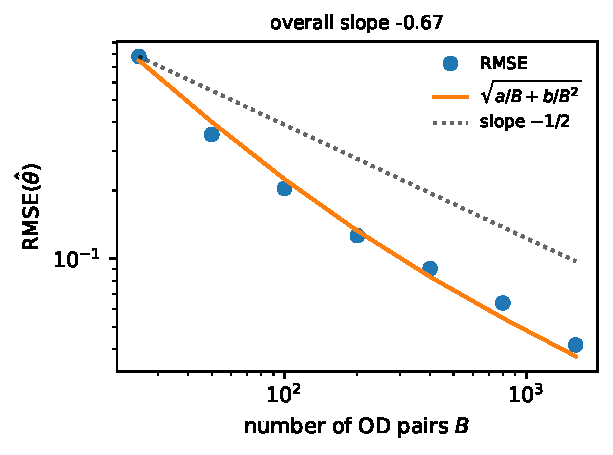
\includegraphics[width=0.52\textwidth]{claim3_synth.pdf}
\caption{Consistency of $\hat\theta$. Root-mean-square error versus the number of
OD pairs $B$ on log--log axes ($D=200$, $L=3$). The fitted $a/B+b/B^2$ curve (with
$b>0$) explains the slightly-steeper-than-$-1/2$ small-$B$ slope; the decay
approaches the $\sqrt B$ rate as $B$ grows.}\label{fig:claim3}
\end{figure}

\paragraph{Identifying the shape coefficients.} The shape coefficients are only
weakly separated, and not in the naive ``higher degree is harder'' way. On the flow
support --- which concentrates near zero, since most links carry almost no flow ---
the monomials $x^l$ that the degrees $l=3,4,5$ multiply are strongly collinear: at
$\theta_0$ the $\gamma$-block score correlations are $0.95$--$0.99$ and the bread
$A$ of the sandwich is ill-conditioned ($\operatorname{cond}(A)\approx 5\times
10^4$). The per-coordinate error in $\hat\gamma_l$ is therefore large and
\emph{non-monotone} in degree --- the cubic term, not the quintic, is the least
stable under the collinearity --- and shrinks only slowly with the data, even
though the joint estimate is $\sqrt B$-consistent and the sandwich variance
correctly reflects the ill-conditioning. Resolving the individual high-degree
coefficients thus demands substantially more data (more OD pairs and more trips per
pair) than the aggregate fit: this is the statistical price of the semiparametric
flexibility, and the reason a parsimonious sieve (small $L$) or a regularized
$\gamma$ is preferable unless the data are rich.

\paragraph{An orthonormal sieve basis.} Part of the conditioning above is an
artifact of the monomial (power-series) parametrization rather than the data: the
shape monomials $\{\xi^3,\dots,\xi^L\}$ have a Hilbert-type Gram matrix on $[0,1]$,
the textbook ill-conditioning of power-series sieves. We therefore also offer a
\emph{fixed} orthonormal parametrization: orthonormalize the shape subspace in
$L^2([0,1])$ (within $\mathrm{span}\{\xi^3,\dots,\xi^L\}$, so the quadratic baseline
is untouched) and parametrize $\gamma = T c$ for a constant invertible $T$. Because
$T$ is a fixed linear map applied only at the estimator boundary -- the forward
solver still receives monomial $\gamma$ -- the falling-factorial U-statistics and
the loss are unchanged and the debiased score merely pulls back by $T^\top$, so
\emph{the debiasing is preserved exactly}: at $\theta_0$ the debiased score remains
mean-zero in the orthonormal basis (the naive plug-in stays biased), as in the
score experiment above, and the Bernstein convexity set carries over as the
polyhedron $\{(MT)c \ge -1\}$. The reparametrization sharply improves the sieve
conditioning: the $\gamma$-block condition number falls from $\approx 3.7\times10^3$
(monomial) to $\approx 50$ (orthonormal), a $\sim\!70\times$ reduction, confirming
that most of the monomial conditioning was basis-induced and removable. The honest
caveat is that the well-identified object is then the \emph{function} (equivalently,
the orthonormal coefficients $c$); the individual \emph{monomial} coefficients
$\gamma_l$ remain weakly identified, because mapping back inflates their variance,
$\operatorname{Var}(\hat\gamma) = T\operatorname{Var}(\hat c)\,T^\top$ -- the
intrinsic, representation-dependent part of the limit. The orthonormal basis is thus
the right space in which to estimate and report the sieve; it does not manufacture
identification of the power-series coefficients that the flow support cannot resolve.

\paragraph{The choice of $\Gamma$.} The parametrization of $\Gamma$ also
matters when the truth has negative curvature corrections. With
$\gamma_0=(0.8,-0.3)$ (in the Bernstein polyhedron $\Gamma_B$ but outside
$\mathbb{R}_+$), the nonnegative parametrization clips $\hat\gamma_4$ to $0$
(RMSE $0.30$, the full bias), whereas the Bernstein parametrization recovers the
negative coefficient ($\hat\gamma_4 \approx -0.31$, RMSE $0.07$; $B=200$, $D=2000$,
$40$ replications). The Bernstein polyhedron is therefore the better default when
the data may favour less curvature than the quadratic baseline.

\paragraph{The inner solver in the estimation loop.} At every $\theta$ visited by
the outer loop the batched interior-point solver converges in a small, essentially
constant number of iterations and matches the independent \textsc{scipy} dual
oracle, as Proposition~\ref{prop:ipm} guarantees. This holds at scale: on Chicago
Sketch ($2\,950$ arcs) across a sweep of $\theta$ values the solver takes $13$--$14$
iterations per $\theta$ and reproduces the per-OD \textsc{scipy} solution to
$5\times10^{-7}$. Because the primal method re-centres from its strictly-interior
start, its iteration count does not depend on a multiplier warm start; the
efficiency of the loop comes instead from solving all OD pairs of a network in a
single vectorized (batched) pass, with the per-iteration arithmetic and the
safeguard line search evaluated by GIL-released native kernels.

\section{Application to Shenzhen taxi data}\label{sec:application}

TBC: Estimate a nice base model with  a nice set of parameters. Show estimates for $L=3,...,\text{something}$. Perhaps do out-of-sample validation with 5-way splits (or 10 if there is a lot of data?). 

\section{Concluding remarks}\label{sec:conclusion}

TBC

\appendix

\section{Eliminating the primal and bound-multiplier directions}
\label{app:ipm-elimination}

This appendix derives the normal equation~\eqref{eq:ipm-normal} and the
back-substitution formulas~\eqref{eq:ipm-backsub}. Start from the linearized KKT
system:
\[
\begin{aligned}
    \operatorname{diag}(\ell\odot h''(x;\gamma))\Delta x
        +C^\top\Delta\lambda-\Delta z+\Delta w &= -r_{\mathrm d},\\
    C\Delta x &= -r_{\mathrm p},\\
    z\odot\Delta x+x\odot\Delta z &= q_z,\\
    -w\odot\Delta x+(\mathbf 1-x)\odot\Delta w &= q_w.
\end{aligned}
\]
All divisions below are elementwise. Since the interior-point iterate satisfies
$0<x<1$ and $z,w>0$, the complementarity equations can be solved coordinate by
coordinate:
\begin{equation}\label{eq:app-dzdw}
    \Delta z=\frac{q_z-z\odot\Delta x}{x},
    \qquad
    \Delta w=\frac{q_w+w\odot\Delta x}{\mathbf 1-x}.
\end{equation}
Substituting~\eqref{eq:app-dzdw} into the stationarity equation gives
\[
\begin{aligned}
&\operatorname{diag}(\ell\odot h''(x;\gamma))\Delta x
    +C^\top\Delta\lambda
    -\frac{q_z-z\odot\Delta x}{x}
    +\frac{q_w+w\odot\Delta x}{\mathbf 1-x}
    =-r_{\mathrm d}.
\end{aligned}
\]
Collecting the terms that multiply $\Delta x$ yields
\[
    \Theta\odot\Delta x+C^\top\Delta\lambda
    =
    -r_{\mathrm d}+\frac{q_z}{x}-\frac{q_w}{\mathbf 1-x}
    =:s,
\]
where
\[
    \Theta_i=\ell_i h''(x_i;\gamma)+\frac{z_i}{x_i}
        +\frac{w_i}{1-x_i}.
\]
Therefore
\begin{equation}\label{eq:app-dx}
    \Delta x=\operatorname{diag}(\Theta)^{-1}(s-C^\top\Delta\lambda).
\end{equation}
Finally, impose the linearized feasibility equation $C\Delta x=-r_{\mathrm p}$:
\[
    C\operatorname{diag}(\Theta)^{-1}(s-C^\top\Delta\lambda)
    =-r_{\mathrm p}.
\]
Rearranging gives the normal equation for the multiplier direction,
\[
    C\operatorname{diag}(\Theta)^{-1}C^\top\Delta\lambda
    =
    r_{\mathrm p}+C\operatorname{diag}(\Theta)^{-1}s.
\]
This is~\eqref{eq:ipm-normal}. Once $\Delta\lambda$ is obtained from this
weighted Laplacian system, $\Delta x$ follows from~\eqref{eq:app-dx}, and then
$(\Delta z,\Delta w)$ follow from~\eqref{eq:app-dzdw}. This is the
back-substitution step~\eqref{eq:ipm-backsub}.

\bibliographystyle{plainnat}
\bibliography{references}

\end{document}
